% chktex-file 2% chktex-file 29
% chktex-file 13
\documentclass{report}
\usepackage{setspace}
\usepackage[a4paper, total={7in, 10in}]{geometry}
\usepackage[fleqn]{amsmath}
\usepackage{empheq}
\usepackage{amssymb}
\usepackage{amsthm}
\usepackage{gensymb}
\usepackage[fleqn]{cases}
\usepackage{multicol}
\usepackage{color}
\usepackage{stix}
\usepackage{chngcntr}
\usepackage{tikz}
\usepackage{enumitem}
\usepackage{pgfplots}
\usepackage{etoolbox}
\usepackage{tikz-3dplot}
\usepackage{tkz-euclide}
\usepackage{graphicx}
\usepackage{enumitem}

\def\nswe#1#2#3{#1\,$#2^\circ\,#3'$}
\graphicspath{ {./assets/} }
\usetikzlibrary{calc,matrix,arrows}
\usetikzlibrary{decorations.pathmorphing,patterns, calligraphy, perspective,backgrounds}

\tikzset{
    right angle quadrant/.code={
            \pgfmathsetmacro\quadranta{{1,1,-1,-1}[#1-1]}     % Arrays for selecting quadrant
            \pgfmathsetmacro\quadrantb{{1,-1,-1,1}[#1-1]}},
    right angle quadrant=1, % Make sure it is set, even if not called explicitly
    right angle length/.code={\def\rightanglelength{#1}},   % Length of symbol
    right angle length=2ex, % Make sure it is set...
    right angle symbol/.style n args={3}{
            insert path={
                    let \p0 = ($(#1)!(#3)!(#2)$) in     % Intersection
                    let \p1 = ($(\p0)!\quadranta*\rightanglelength!(#3)$), % Point on base line
                    \p2 = ($(\p0)!\quadrantb*\rightanglelength!(#2)$) in % Point on perpendicular line
                    let \p3 = ($(\p1)+(\p2)-(\p0)$) in  % Corner point of symbol
                    (\p1) -- (\p3) -- (\p2)
                }
        }
}

\counterwithout{equation}{chapter}
\setlength{\columnseprule}{1pt}
\setlength{\columnsep}{24pt}
\setcounter{chapter}{16}
\hfuzz=100pt

\newcommand{\pgfplotsdrawaxis}{\pgfplots@draw@axis}
\makeatother
\pgfplotsset{only axis on top/.style={axis on top=false, after end axis/.code={
                    \pgfplotsset{axis line style=opaque, ticklabel style=opaque, tick style={thick,opaque},
                        grid=none}\pgfplotsdrawaxis}}}

\newtheorem{theorem}{Theorem}

\begin{document}\makeatletter
\newcommand{\newparallel}{\mathrel{\mathpalette\new@parallel\relax}}
\newcommand{\new@parallel}[2]{%
    \begingroup
    \sbox\z@{$#1T$}% get the height of an uppercase letter
    \resizebox{!}{\ht\z@}{\raisebox{\depth}{$\m@th#1/\mkern-5mu/$}}%
    \endgroup
}
\makeatother

\newcommand{\planelineinter}[5]% a, b, c, p as {a_x,a_y,a_z}, coordinate name
{   \foreach \a [count=\k] in {#1}
        { \ifthenelse{\k=1}{\xdef\tempxa{\a}}
            \ifthenelse{\k=2}{\xdef\tempya{\a}}
            \ifthenelse{\k=3}{\xdef\tempza{\a}}
        }
    \foreach \b [count=\k] in {#2}
        { \ifthenelse{\k=1}{\xdef\tempxb{\b}}
            \ifthenelse{\k=2}{\xdef\tempyb{\b}}
            \ifthenelse{\k=3}{\xdef\tempzb{\b}}
        }
    \foreach \c [count=\k] in {#3}
        { \ifthenelse{\k=1}{\xdef\tempxc{\c}}
            \ifthenelse{\k=2}{\xdef\tempyc{\c}}
            \ifthenelse{\k=3}{\xdef\tempzc{\c}}
        }
    \foreach \p [count=\k] in {#4}
        { \ifthenelse{\k=1}{\xdef\tempxp{\p}}
            \ifthenelse{\k=2}{\xdef\tempyp{\p}}
            \ifthenelse{\k=3}{\xdef\tempzp{\p}}
        }
    \pgfmathsetmacro{\abx}{\tempxb-\tempxa}
    \pgfmathsetmacro{\aby}{\tempyb-\tempya}
    \pgfmathsetmacro{\abz}{\tempzb-\tempza}
    \pgfmathsetmacro{\acx}{\tempxc-\tempxa}
    \pgfmathsetmacro{\acy}{\tempyc-\tempya}
    \pgfmathsetmacro{\acz}{\tempzc-\tempza}
    \pgfmathsetmacro{\nx}{\aby*\acz-\abz*\acy}
    \pgfmathsetmacro{\ny}{\abz*\acx-\abx*\acz}
    \pgfmathsetmacro{\nz}{\abx*\acy-\aby*\acx}
    \pgfmathsetmacro{\d}{(\nx+\ny+\nz)/(\nx*\tempxp+\ny*\tempyp+\nz*\tempzp)}
    \path (0,0,0) -- (#4) coordinate[pos=\d] (#5);
}

% golden ratio and inverse golden ratio
\pgfmathsetmacro{\gr}{(1+sqrt(5))/2}
\pgfmathsetmacro{\igr}{2/(1+sqrt(5))}

%choose axis angles
\newcommand{\xangle}{0}
\newcommand{\yangle}{90}
\newcommand{\zangle}{225}

%choose axis lengths
\newcommand{\xlength}{1}
\newcommand{\ylength}{1}
\newcommand{\zlength}{0.5}

\pgfmathsetmacro{\xx}{\xlength*cos(\xangle)}
\pgfmathsetmacro{\xy}{\xlength*sin(\xangle)}
\pgfmathsetmacro{\yx}{\ylength*cos(\yangle)}
\pgfmathsetmacro{\yy}{\ylength*sin(\yangle)}
\pgfmathsetmacro{\zx}{\zlength*cos(\zangle)}
\pgfmathsetmacro{\zy}{\zlength*sin(\zangle)}

\newcommand{\sol}[1]{

    \noindent \textbf{Sol.}
}
\newcommand{\prooff}[1]{

    \noindent \textbf{Proof.}
}
\newcommand\m[1]{\begin{pmatrix}#1\end{pmatrix}}
\newcommand\vm[1]{\begin{vmatrix}#1\end{vmatrix}}
\newenvironment{amatrix}[1]{%
    \left(\begin{array}{@{}*{#1}{c}|c@{}}
        }{%
    \end{array}\right)
}
\newenvironment{cequation}{
    \makeatletter
    \setbool{@fleqn}{false}
    \makeatother
    \begin{equation*}
        }{\end{equation*}}

\begin{titlepage}
    \raggedleft{}
    \rule{1pt}{\textheight}
    \hspace{0.02\textwidth}
    \parbox[b]{0.75\textwidth}{

    {\Huge\bfseries Solution Book of \\[0.5\baselineskip] Mathematic}\\[2\baselineskip]
    {\large\textit{Ssnior 2 Part I}}\\[4\baselineskip]
    {\Large\textsc{MELVIN CHIA}}

    \vspace{0.5\textheight}

    {\noindent Written on 9 October 2022}\\[\baselineskip]
    }

\end{titlepage}

\doublespacing{}
\tableofcontents
\singlespacing{}
\newpage

\appendix
\chapter{Cheat Sheet}
\begin{multicols}{2}
    \setcounter{section}{11}
    \section{Sequence and Series}

    \begin{enumerate}
        \item Series:
              \begin{enumerate}
                  \item Finite series: $a_1 + a_2 + a_3 + \cdots + a_n = \sum_{k=1}^n a_k$
                  \item Infinite series: $a_1 + a_2 + a_3 + \cdots = \sum_{k=1}^\infty a_k$
              \end{enumerate}
        \item General term:
              \begin{enumerate}
                  \item Arithmetic sequence: $a_n = a_1 + (n-1)d$
                  \item Geometric sequence: $a_n = a_1 r^{n-1}$
              \end{enumerate}
        \item Summation formula:
              \begin{enumerate}
                  \item Arithmetic sequence:
                        \begin{enumerate}
                            \item $S_n = \frac{1}{2}n(a_1 + a_n)$
                            \item $S_n = \frac{n}{2}[2a_1 + (n-1)d]$
                        \end{enumerate}
                  \item Geometric sequence:
                        \begin{enumerate}
                            \item When $r \neq 1$: $S_n = \frac{a_1(1-r^n)}{1-r}$
                            \item When $r = 1$: $S_n = na_1$
                        \end{enumerate}
              \end{enumerate}
        \item Mean:
              \begin{enumerate}
                  \item Arithmetic mean: $A = {x+y}{2}$
                  \item Geometric mean: $G = \pm\sqrt{xy}$
              \end{enumerate}
        \item Summation of infinite geometric series: \[S = \frac{a_1}{1-r} \quad (1 < r < 1)\]
        \item Simple summation formulas:
              \begin{enumerate}
                  \item $\sum_{k=1}^n k = \frac{n(n+1)}{2}$
                  \item $\sum_{k=1}^n k^2 = \frac{n(n+1)(2n+1)}{6}$
                  \item $\sum_{k=1}^n k^3 = \frac{n^2(n+1)^2}{4}$
              \end{enumerate}
    \end{enumerate}

    \setcounter{section}{13}
    \section{Matrices and Determinants}

    \begin{enumerate}
        \item General form of matrix: $A = \m{a_{11} & a_{12} & \cdots & a_{1n} \\ a_{21} &
                      a_{22} & \cdots & a_{2n} \\ \vdots & \vdots & \ddots & \vdots \\ a_{m1} &
                      a_{m2} & \cdots & a_{mn}}$
        \item Square matrix: $\m{a_{11} & a_{12} & \cdots & a_{1n} \\ a_{21} & a_{22} &
                      \cdots & a_{2n} \\ \vdots & \vdots & \ddots & \vdots \\ a_{n1} & a_{n2} &
                      \cdots & a_{nn}}$
        \item Zero matrix: $A = \m{0 & 0 & \cdots & 0 \\ 0 & 0 & \cdots & 0 \\ \vdots &
                      \vdots & \ddots & \vdots \\ 0 & 0 & \cdots & 0}$
        \item Identity matrix: $I = \m{1 & 0 & \cdots & 0 \\ 0 & 1 & \cdots & 0 \\ \vdots &
                      \vdots & \ddots & \vdots \\ 0 & 0 & \cdots & 1}$
        \item Transpose of a matrix: $A' = \m{a_{11} & a_{21} & \cdots & a_{m1} \\ a_{12} &
                      a_{22} & \cdots & a_{m2} \\ \vdots & \vdots & \ddots & \vdots \\ a_{1n} &
                      a_{2n} & \cdots & a_{mn}}$
        \item Addition of matrices: $A + B = \m{ a_{11} + b_{11} & a_{12} + b_{12}\\ a_{21} +
                      b_{21} & a_{22} + b_{22} }$
        \item Subtraction of matrices: $A - B = \m{ a_{11} - b_{11} & a_{12} - b_{12}\\
                      a_{21} - b_{21} & a_{22} - b_{22} }$
        \item Properties of addition and subtraction of matrices:
              \begin{enumerate}
                  \item $A + B = B + A$
                  \item $(A + B) + C = A + (B + C)$
                  \item $A + O = A$
                  \item $(A \pm B)' = A' \pm B'$
              \end{enumerate}
        \item Scalar product of a matrix: $kA = \m{ka_{11} & ka_{12} \\ ka_{21} & ka_{22}}$
        \item Multiplication of matrices: $(AB)_{ij} = \sum_{k=1}^n a_{ik}b_{kj}$
        \item Properties of multiplication of matrices:
              \begin{enumerate}
                  \item $A(BC) = (AB)C$
                  \item $A(B + C) = AB + AC$
                  \item $(B+C)A = BA + CA$
                  \item $k(AB) = A(kB)$
                  \item $(AB)' = B'A'$
              \end{enumerate}
        \item Determinants:
              \begin{enumerate}
                  \item $2\times 2$ determinant: $\det(A) = \begin{vmatrix}
                                a & b \\
                                c & d
                            \end{vmatrix} = ad - bc$
                  \item $3\times 3$ determinant:
                        \begin{flalign*}
                            \det(A) & = \vm{
                            a_1     & b_1                                             & c_1 \\
                            a_2     & b_2                                             & c_2 \\
                            a_3     & b_3                                             & c_3
                            }       &                                                       \\
                                    & = a_1\vm{
                            b_2     & c_2                                                   \\
                            b_3     & c_3
                            } - b_1\vm{
                            a_2     & c_2                                                   \\
                            a_3     & c_3
                            } + c_1\vm{
                            a_2     & b_2                                                   \\
                            a_3     & b_3
                            }                                                               \\
                                    & = a_1b_2c_3 + b_1c_2a_3 + c_1a_2b_3 - a_3b_2c_1       \\
                                    & \ \ \ \ - b_3c_2a_1 - c_3a_2b_1
                        \end{flalign*}
              \end{enumerate}
        \item The Sarrus method:
              \begin{center}
                  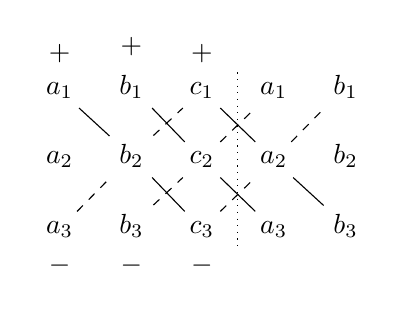
\begin{tikzpicture}
                      \matrix [%
                          matrix of math nodes,
                          column sep=1em,
                          row sep=1em
                      ] (sarrus) {%
                          a_1 & b_1 & c_1 & a_1 & b_1 \\
                          a_2 & b_2 & c_2 & a_2 & b_2 \\
                          a_3 & b_3 & c_3 & a_3 & b_3 \\
                      };

                      \path ($(sarrus-1-3.north east)+(0.5em,0)$) edge[dotted] ($(sarrus-3-3.south east)+(0.5em,0)$)
                      (sarrus-1-1)                          edge         (sarrus-2-2)
                      (sarrus-2-2)                          edge         (sarrus-3-3)
                      (sarrus-1-2)                          edge         (sarrus-2-3)
                      (sarrus-2-3)                          edge         (sarrus-3-4)
                      (sarrus-1-3)                          edge         (sarrus-2-4)
                      (sarrus-2-4)                          edge         (sarrus-3-5)
                      (sarrus-3-1)                          edge[dashed] (sarrus-2-2)
                      (sarrus-2-2)                          edge[dashed] (sarrus-1-3)
                      (sarrus-3-2)                          edge[dashed] (sarrus-2-3)
                      (sarrus-2-3)                          edge[dashed] (sarrus-1-4)
                      (sarrus-3-3)                          edge[dashed] (sarrus-2-4)
                      (sarrus-2-4)                          edge[dashed] (sarrus-1-5);

                      \foreach \c in {1,2,3} {\node[anchor=south] at (sarrus-1-\c.north) {$+$};};
                      \foreach \c in {1,2,3} {\node[anchor=north] at (sarrus-3-\c.south) {$-$};};
                  \end{tikzpicture}
              \end{center}
        \item Minor of an element in a matrix: the determinant of the matrix obtained by
              removing the row and column containing the element
        \item Cofactor of an element in a matrix: the minor of the element multiplied by
              $(-1)^{i+j}$
        \item Theorems of $3\times 3$ determinants:
              \begin{theorem}
                  The determinant of a 3x3 matrix is the sum of the elements of any row or
                  column multiplied by the cofactors of the elements of that row or column.
                  \begin{flalign*}
                      \vm{A} & = a_1A_1 + b_1B_1 + c_1C_1 \\
                             & = a_2B_2 + b_2B_2 + c_2C_2 \\
                             & = a_3C_3 + b_3C_3 + c_3C_3 \\
                             & = a_1A_1 + a_2A_2 + a_3A_3 \\
                             & = b_1B_1 + b_2B_2 + b_3B_3 \\
                             & = c_1C_1 + c_2C_2 + c_3C_3
                  \end{flalign*}
              \end{theorem}
              \begin{theorem}
                  The product of the elements of any row or column and the cofactor of corresponding elements of another row or column of a determinant is 0.
                  \begin{flalign*}
                       & a_2B_1 + b_2B_1 + c_2C_1                                          \\
                       & = a_2\vm{ b_2                                               & c_2 \\ b_3 & c_3 } - b_2\vm{ a_2 & c_2 \\ a_3 & c_3 } + c_2\vm{ a_2 & b_2 \\ a_3 & b_3 } \\
                       & = a_2b_2c_3 + a_2b_3c_2 - a_2b_2c_3 + a_3b_2c_2 + a_2b_3c_2       \\
                       & \ \ \ \ - a_3b_2c_2                                               \\
                       & = 0
                  \end{flalign*}
              \end{theorem}
        \item Identities of determinants: \setcounter{theorem}{0}
              \begin{theorem}
                  The value of a determinant is the same as the value of its transpose, aka $|A| = |A'|$.
                  \begin{cequation}
                      \vm{ a & b \\ c & d } = \vm{ a & c \\ b & d }
                  \end{cequation}
              \end{theorem}
              \begin{theorem}
                  Switching any two rows or columns of a determinants results in the opposite value.
                  \begin{cequation}
                      \vm{ a_1 & b_1 & c_1 \\ a_2 & b_2 & c_2 \\ a_3 & b_3 & c_3 } = -\vm{ a_1 & b_1 & c_1 \\ a_3 & b_3 & c_3 \\ a_2 & b_2 & c_2 }
                  \end{cequation}
              \end{theorem}
              \begin{theorem}
                  If two rows or cols of a determinant are identical, the value of the determinant is zero.
                  \begin{cequation}
                      \vm{ a & b & c \\ a & b & c \\ d & e & f } = 0 \\
                  \end{cequation}
              \end{theorem}
              \begin{theorem}
                  If all elements of a row (or column) of a determinant are multiplied by some scalar number k, the value of the new determinant is k times of the given determinant.
                  \begin{cequation}
                      \vm{ a_1 & b_1 & c_1 \\ ka_2 & kb_2 & kc_2 \\ a_3 & b_3 & c_3 } = k\vm{ a_1 & b_1 & c_1 \\ a_2 & b_2 & c_2 \\ a_3 & b_3 & c_3 }
                  \end{cequation}
              \end{theorem}
              \begin{theorem}
                  In a determinant each element in any row (or column) consists of the sum of two terms, then the determinant can be expressed as sum of two determinants of same order.
                  \begin{cequation}
                      \vm{ a_1+d_1 & b_1 & c_1 \\ a_2+d_2 & b_2 & c_2 \\ a_3+d_3 & b_3 & c_3 } = \vm{ a_1 & b_1 & c_1 \\ a_2 & b_2 & c_2 \\ a_3 & b_3 & c_3 } + \vm{ d_1 & b_1 & c_1 \\ d_2 & b_2 & c_2 \\ d_3 & b_3 & c_3 }
                  \end{cequation}
              \end{theorem}
              \begin{theorem}
                  If a determinant is obtained by adding a row or column multiplied by a some scalar number k to a different row or column, then the value of the new determinant is the same as the original determinant.
                  \begin{cequation}
                      \vm{ a_1 & b_1 & c_1 \\ a_2 & b_2 & c_2 \\ a_3 & b_3 & c_3 } = \vm{ a_1+ka_2 & b_1+kb_2 & c_1+kc_2 \\ a_2 & b_2 & c_2 \\ a_3 & b_3 & c_3 }
                  \end{cequation}
              \end{theorem}
              \begin{theorem}
                  The determinant of product of two matrices of equal size is equal to the product of determinants of each matrix, aka $|AB| = |A||B|$.
              \end{theorem}
        \item Inverse of a matrix:
              \begin{enumerate}
                  \item $AB = BA = I$
                  \item $B = A^{-1}$, $A = B^{-1}$
              \end{enumerate}
        \item Formulas of inverse matrix:
              \begin{enumerate}
                  \item Inverse of a $2\times 2$ matrix: $A^{-1} = \frac{1}{ad-bc}\vm{ d & -b \\ -c & a
                            }$
                  \item Inverse of a $3\times 3$ matrix: $A^{-1} = \frac{1}{|A|} \operatorname{adj}A$
              \end{enumerate}
        \item Adjoint of a matrix: \[\operatorname{adj}\m{ a_1 & b_1 & c_1 \\ a_2 & b_2 & c_2
                      \\ a_3 & b_3 & c_3 } = \m{A_1& A_2& A_3 \\ B_1& B_2& B_3 \\ C_1& C_2& C_3}\]
        \item Gauss elimination:
              \begin{enumerate}
                  \item Interchange two rows:

                        $R_i \leftrightarrow R_j$: interchange row $i$ and row
                        $j$.
                  \item Multiply a row by a nonzero constant:

                        $R_i \rightarrow kR_i$: multiply row $i$
                        by $k$, where $k$ is a nonzero constant.
                  \item Add a multiple of one row to another row:

                        $R_i \rightarrow R_i + kR_j$: add $k$ times row
                        $j$ to row $i$.
              \end{enumerate}
        \item Inverse a matrix with Gauss elimination:
              \begin{flalign*}
                         & \left(\begin{array}{ccc|ccc}
                                     a_{11} & a_{12} & a_{13} & 1 & 0 & 0 \\
                                     a_{21} & a_{22} & a_{23} & 0 & 1 & 0 \\
                                     a_{31} & a_{32} & a_{33} & 0 & 0 & 1
                                 \end{array}\right)
                  \\                                 & \Rightarrow
                  \left(\begin{array}{ccc|ccc}
                            1 & 0 & 0 & b_{11} & b_{12} & b_{13} \\
                            0 & 1 & 0 & b_{21} & b_{22} & b_{23} \\
                            0 & 0 & 1 & b_{31} & b_{32} & b_{33}
                        \end{array}\right)                       \\
                  A^{-1} & = \m{ b_{11}                                              & b_{12} & b_{13} \\ b_{21} & b_{22} & b_{23} \\ b_{31} & b_{32} & b_{33} }
              \end{flalign*}
        \item Cramer's Rule:
              \begin{flalign*}
                  \begin{cases}
                      a_1x + b_1y + c_1z = d_1 \\
                      a_2x + b_2y + c_2z = d_2 \\
                      a_3x + b_3y + c_3z = d_3
                  \end{cases} \\\\
                  \Delta = \m{
                  a_1 & b_1 & c_1                             \\
                  a_2 & b_2 & c_2                             \\
                  a_3 & b_3 & c_3
                  }                                           \\
                  \Delta_x = \m{
                  d_1 & b_1 & c_1                             \\
                  d_2 & b_2 & c_2                             \\
                  d_3 & b_3 & c_3
                  }
                  \\
                  \Delta_y = \m{
                  a_1 & d_1 & c_1                             \\
                  a_2 & d_2 & c_2                             \\
                  a_3 & d_3 & c_3
                  }
                  \\
                  \Delta_z = \m{
                  a_1 & b_1 & d_1                             \\
                  a_2 & b_2 & d_2                             \\
                  a_3 & b_3 & d_3
                  }                                           \\\\
                  x = \frac{\Delta_x}{\Delta}                 ,\
                  y = \frac{\Delta_y}{\Delta}                 ,\
                  z = \frac{\Delta_z}{\Delta}
              \end{flalign*}
    \end{enumerate}

    \section{Inequalities}

    \begin{enumerate}
        \item Inequalities signs:
              \begin{enumerate}
                  \item $<$: less than
                  \item $>$: greater than
                  \item $\leq$: less than or equal to
                  \item $\geq$: greater than or equal to
              \end{enumerate}
        \item Compare numbers by their difference:
              \begin{enumerate}
                  \item If $a - b > 0$, then $a > b$
                  \item If $a - b < 0$, then $a < b$
              \end{enumerate}
        \item Identities of inequalities: \setcounter{theorem}{0}
              \begin{theorem}
                  If $a > b$, $b > c$, then $a > c$
              \end{theorem}
              \begin{theorem}
                  If $a > b$ then $a + c > b + c$
              \end{theorem}
              \begin{theorem}
                  If $a > b$, $c > d$, then $a + c > b + d$
              \end{theorem}
              \begin{theorem}
                  If $a > b$, then:
                  \begin{enumerate}
                      \item When $c > 0$, $ac > bc$
                      \item When $c = 0$, $ac = bc$
                      \item When $c < 0$, $ac < bc$
                  \end{enumerate}
              \end{theorem}
    \end{enumerate}
\end{multicols}
\end{document}